% Generated by Listas/make_statements.py from pratica-lecture-06.md, item 15. Do not edit.
\textbf{Source.} Tadelis (2013), \emph{Game Theory: An Introduction}, Exercise 10.4 ``Trust Off the Equilibrium Path'', p.~216 {[}PDF 235{]}. Reproduced verbatim. Figure 10.1 (p.~205) is not part of the exercise text; it is added because the statement refers to it. Answer in the source: none in the book (the preface, p.~xiii, says about half are solved on Princeton UP's website; not checked).



\begin{quote}

\textbf{Trust Off the Equilibrium Path:} Recall the trust game depicted in Figure 10.1. We argued that for \(\delta \ge \frac{1}{2}\) the following pair of strategies is a subgame-perfect equilibrium. For player 1: ``In period 1 I will trust player 2, and as long as there were no deviations from the pair \((T, C)\) in any period, then I will continue to trust him. Once such a deviation occurs then I will not trust him forever after.'' For player 2: ``In period 1 I will cooperate, and as long as there were no deviations from the pair \((T, C)\) in any period, then I will continue to do so. Once such a deviation occurs then I will deviate forever after.'' Show that if instead player 2 uses the strategy ``as long as player 1 trusts me I will cooperate'' then the path \((T, C)\) played forever is a Nash equilibrium for \(\delta \ge \frac{1}{2}\) but is not a subgame-perfect equilibrium for any value of \(\delta\).

\end{quote}



\pandocbounded{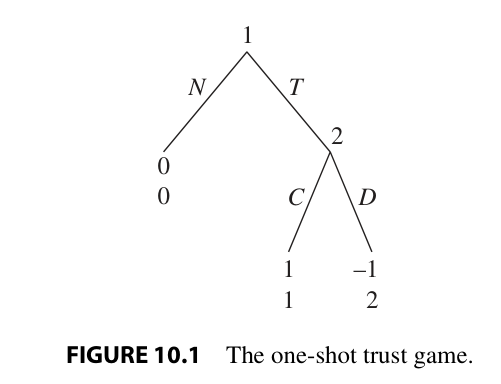
\includegraphics[keepaspectratio,alt={Tadelis Figure 10.1, the one-shot trust game}]{../figures/tadelis-fig-10-1.png}}



\emph{Figure 10.1} The one-shot trust game (Tadelis p.~205; added for reference).

